% Options for packages loaded elsewhere
\PassOptionsToPackage{unicode}{hyperref}
\PassOptionsToPackage{hyphens}{url}
%
\documentclass[
]{article}
\usepackage{amsmath,amssymb}
\usepackage{iftex}
\ifPDFTeX
  \usepackage[T1]{fontenc}
  \usepackage[utf8]{inputenc}
  \usepackage{textcomp} % provide euro and other symbols
\else % if luatex or xetex
  \usepackage{unicode-math} % this also loads fontspec
  \defaultfontfeatures{Scale=MatchLowercase}
  \defaultfontfeatures[\rmfamily]{Ligatures=TeX,Scale=1}
\fi
\usepackage{lmodern}
\ifPDFTeX\else
  % xetex/luatex font selection
\fi
% Use upquote if available, for straight quotes in verbatim environments
\IfFileExists{upquote.sty}{\usepackage{upquote}}{}
\IfFileExists{microtype.sty}{% use microtype if available
  \usepackage[]{microtype}
  \UseMicrotypeSet[protrusion]{basicmath} % disable protrusion for tt fonts
}{}
\makeatletter
\@ifundefined{KOMAClassName}{% if non-KOMA class
  \IfFileExists{parskip.sty}{%
    \usepackage{parskip}
  }{% else
    \setlength{\parindent}{0pt}
    \setlength{\parskip}{6pt plus 2pt minus 1pt}}
}{% if KOMA class
  \KOMAoptions{parskip=half}}
\makeatother
\usepackage{xcolor}
\usepackage[margin=1in]{geometry}
\usepackage{graphicx}
\makeatletter
\def\maxwidth{\ifdim\Gin@nat@width>\linewidth\linewidth\else\Gin@nat@width\fi}
\def\maxheight{\ifdim\Gin@nat@height>\textheight\textheight\else\Gin@nat@height\fi}
\makeatother
% Scale images if necessary, so that they will not overflow the page
% margins by default, and it is still possible to overwrite the defaults
% using explicit options in \includegraphics[width, height, ...]{}
\setkeys{Gin}{width=\maxwidth,height=\maxheight,keepaspectratio}
% Set default figure placement to htbp
\makeatletter
\def\fps@figure{htbp}
\makeatother
\setlength{\emergencystretch}{3em} % prevent overfull lines
\providecommand{\tightlist}{%
  \setlength{\itemsep}{0pt}\setlength{\parskip}{0pt}}
\setcounter{secnumdepth}{-\maxdimen} % remove section numbering
\ifLuaTeX
  \usepackage{selnolig}  % disable illegal ligatures
\fi
\usepackage{bookmark}
\IfFileExists{xurl.sty}{\usepackage{xurl}}{} % add URL line breaks if available
\urlstyle{same}
\hypersetup{
  pdftitle={Lab 1 Clustering Group 10},
  pdfauthor={Liuxi Mei; Xiaochen Liu},
  hidelinks,
  pdfcreator={LaTeX via pandoc}}

\title{Lab 1 Clustering Group 10}
\author{Liuxi Mei \and Xiaochen Liu}
\date{2025-02-03}

\begin{document}
\maketitle

\subsection{SimpleKmeans}\label{simplekmeans}

Apply ``SimpleKMeans'' to your data. In Weka euclidian distance is
implemented in SimpleKmeans. You can set the number of clusters and seed
of a random algorithm for generating initial cluster centers. Experiment
with the algorithm as follows:

\begin{enumerate}
\def\labelenumi{\arabic{enumi})}
\tightlist
\item
  Choose a set of attributes for clustering and give a motivation.
  (Hint: always ignore attribute ``name''. Why does the name attribute
  need to be ignored?)
\end{enumerate}

The set is chosen is the attributes excluding attributes `Names',
`Protein', and `Fat'. The reason for excluding `Protein' and `Iron' data
is that they both have quite similar mean values across clusters, see
picture below , which means that the differences among cluster are
insignificant and contribute quite less to clustering results.

\begin{figure}
\centering
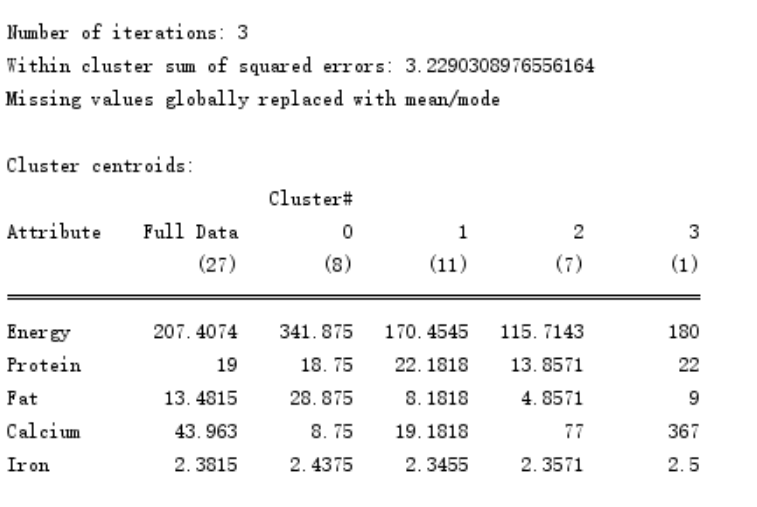
\includegraphics[width=5.20833in,height=\textheight]{Pictures/1.png}
\caption{Clustering result with all numeric attributes}
\end{figure}

`Name' is also ignored as it is a string attribute. For clustering,
Euclidean distance can not be calculated for strings and Weka will also
report a mistake.

\begin{enumerate}
\def\labelenumi{\arabic{enumi})}
\setcounter{enumi}{1}
\item
  Experiment with at least two different numbers of clusters, e.g.~2 and
  5, but with the same seed value 10.

  \begin{figure}
  \centering
  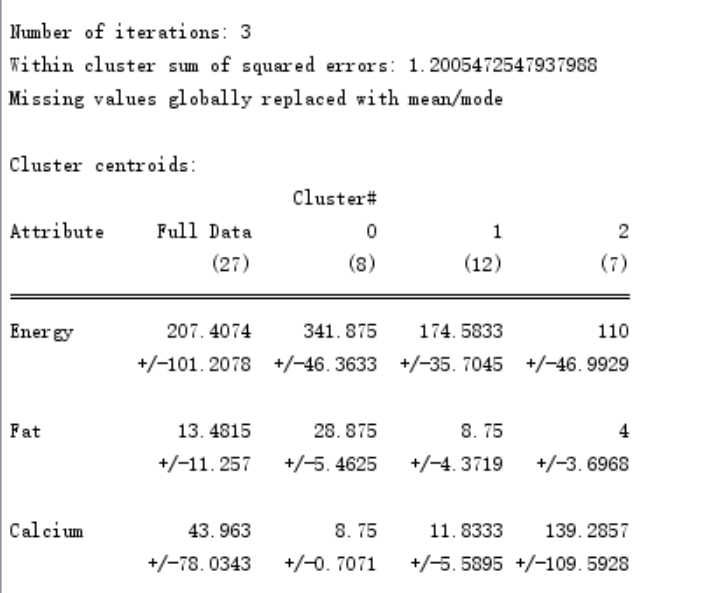
\includegraphics[width=5.20833in,height=\textheight]{Pictures/2.png}
  \caption{Calculated results with 3 clusters, seed set to 10}
  \end{figure}

  \begin{figure}
  \centering
  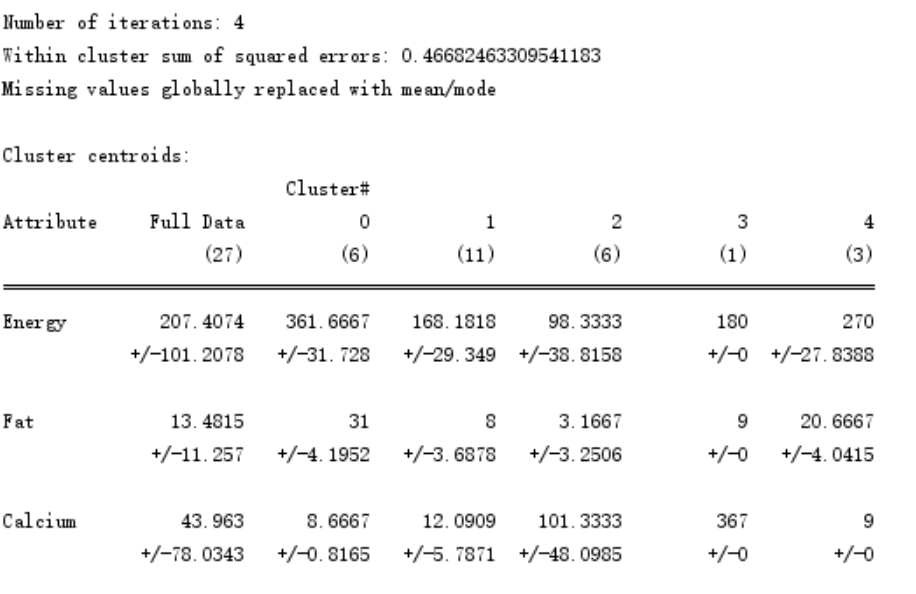
\includegraphics[width=6.25in,height=\textheight]{Pictures/3.png}
  \caption{Calculated results with 5 clusters, seed set to 10}
  \end{figure}
\item
  Then try with a different seed value, i.e.~different initial cluster
  centers. Compare the results with the previous results. Explain what
  the seed value controls.

  With seed = 20, following results are given. Both the numbers of
  instances in clusters and the instances belong to clusters have
  changed. As a result, the variance and mean value for each cluster are
  different from the previous results.

  When initializing this algorithm, N (corresponding to cluster number)
  initial `means' are generated randomly within the data domain, which
  is controlled by the seed number. Different seeds give different
  initial `means', resulting different results in this case.

  \begin{figure}
  \centering
  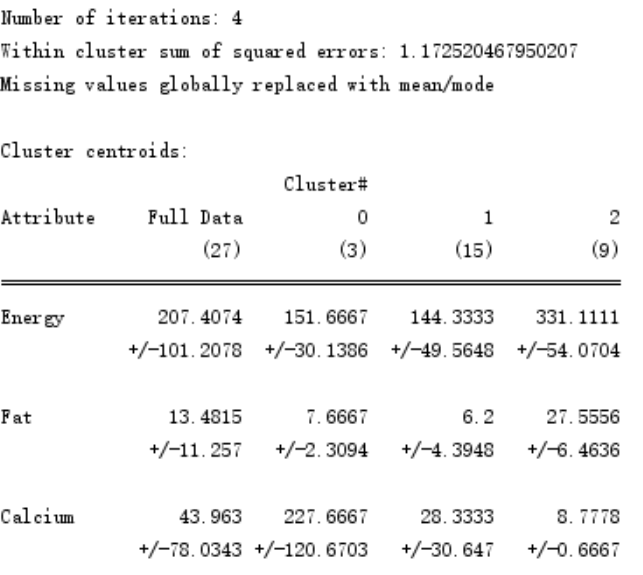
\includegraphics[width=5.20833in,height=\textheight]{Pictures/4.png}
  \caption{Calculated results with 3 clusters, seed set to 20}
  \end{figure}

  \begin{figure}
  \centering
  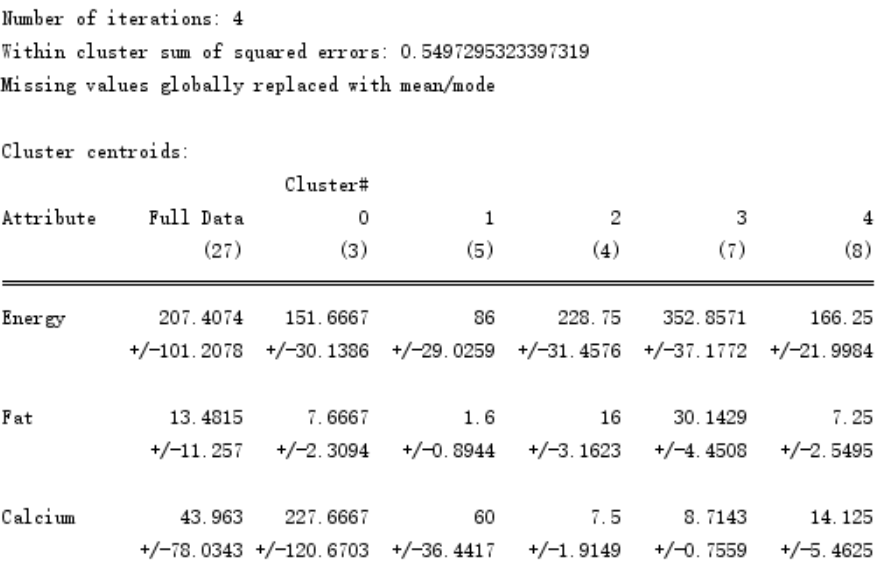
\includegraphics[width=6.25in,height=\textheight]{Pictures/5.png}
  \caption{Calculated results with 5 clusters, seed set to 20}
  \end{figure}
\item
  Do you think the clusters are ``good'' clusters? (Are all of its
  members ``similar'' to each other? Are members from different clusters
  dissimilar?)
\end{enumerate}

Those are not `good' clusters, at least not appropriate for the
application of SimpleKmeans method. If they are obviously similar to
each other, the clusters should include the same instances despite
different seed values.

By applying `standardize' filter to raw data and with seed set to 20,
the regenerated results are shown as the figures below. When cluster
number is chosen to be 3, cluster 0 and 1 different calcium values but
very similar Energy and Fat values. And cluster 2 seems to be a more
independent. For 5 clusters, cluster 0 and 4 are similar in Energy and
Fat values but unsimilar calcium values. The similarity in calcium
values is also noticed between cluster 0 and 1.

\begin{figure}
\centering
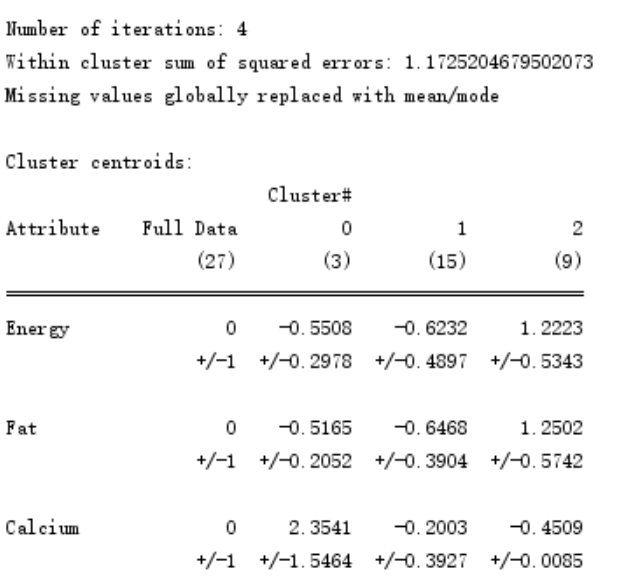
\includegraphics[width=5.20833in,height=\textheight]{Pictures/6.png}
\caption{Calculated results with 3 clusters, seed set to 20, with
standardized data}
\end{figure}

\begin{figure}
\centering
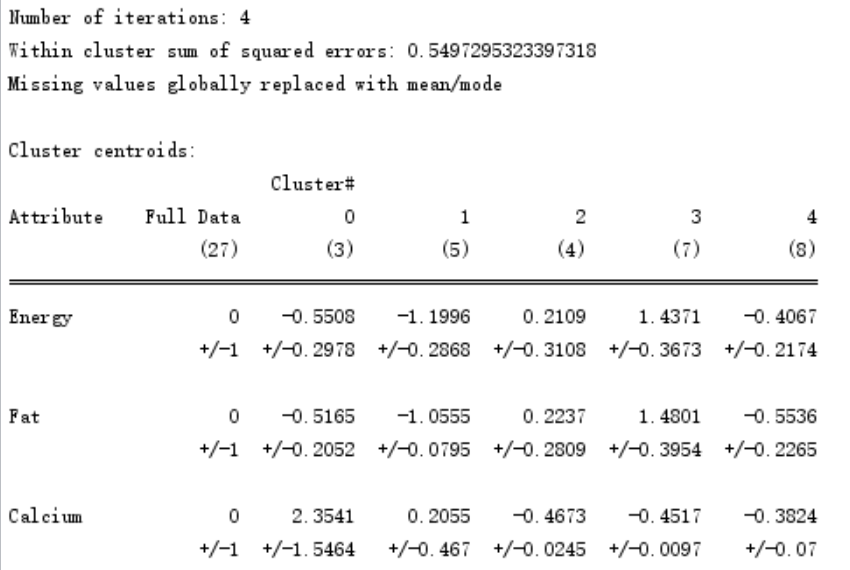
\includegraphics[width=6.25in,height=\textheight]{Pictures/7.png}
\caption{Calculated results with 5 clusters, seed set to 20, with
standardized data}
\end{figure}

\begin{enumerate}
\def\labelenumi{\arabic{enumi})}
\setcounter{enumi}{4}
\tightlist
\item
  What does each cluster represent? Choose one of the results. Make up
  labels (words or phrases in English) which characterize each cluster.
\end{enumerate}

Take figure 6 as an example, cluster 0 is the one with moderate energy,
moderate fat and high calcium level. Cluster 1 is the one with moderate
energy, moderate fat and low calcium level. Cluster 3 is the one with
high energy, high fat and moderate energy level.

\subsection{MakeDensityBasedClusters}\label{makedensitybasedclusters}

Now with MakeDensityBasedClusters, SimpleKMeans is turned into a
density-based cluster. You can set the minimum standard deviation for
normal density calculation. Experiment with the algorithm as the
follows:

\begin{enumerate}
\def\labelenumi{\arabic{enumi})}
\item
  Use the SimpleKMeans clusterer which gave the result you haven chosen
  in 5).
\item
  Experiment with at least two different standard deviations. Compare
  the results. (Hint: Increasing the standard deviation to higher values
  will make the differences in different runs more obvious and thus it
  will be easier to conclude what the parameter does)

  With 0.001 and 0.5 selected for minStdDev, the same cluster centroids
  for 2 custers are initilized, see figure 8. However, the fitted
  cluster vary and cluster have 9 and 8 instances when the minStdDev is
  0.001 and 0.5 respectively. The standard deviations for fitted normal
  distribution models are also different to fulfill the setting of
  minStdDev. As a result, log likelihood is -1.7 for the model with
  0.001 minStdDev and 3.8 for the other.

  \begin{figure}
  \centering
  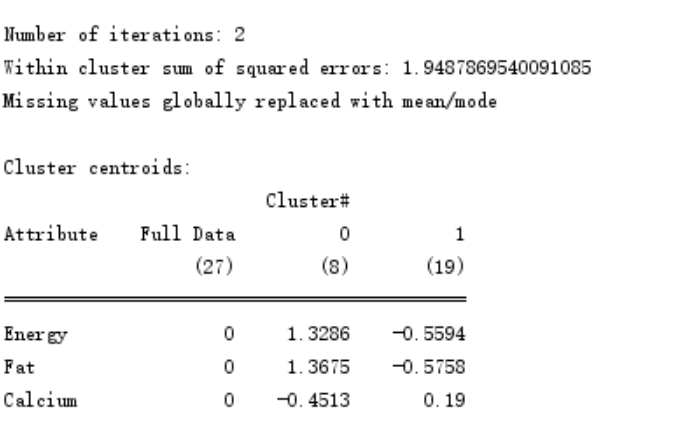
\includegraphics[width=6.25in,height=\textheight]{Pictures/8.png}
  \caption{Initial clusters with cebtroids with MakeDensityBasedClusters
  applied}
  \end{figure}
\end{enumerate}

\end{document}
